%%% Copyright (C) 2018 Vincent Goulet
%%%
%%% Ce fichier fait partie du projet
%%% «Rédaction avec LaTeX»
%%% http://github.com/vigou3/formation-latex-ul
%%%
%%% Cette création est mise à disposition selon le contrat
%%% Attribution-Partage dans les mêmes conditions 4.0
%%% International de Creative Commons.
%%% http://creativecommons.org/licenses/by-sa/4.0/

\chapter{Présentation de {\TeX} et {\LaTeX}}
\label{chap:presentation}

La production d'un document à l'aide d'un ordinateur comprend toujours
trois grandes étapes:
\begin{enumerate}
\item la saisie du texte dans l'ordinateur;
\item la composition du texte sur la page en lignes de longueur égale
  et en paragraphes, ainsi que la disposition des éléments tels que les
  figures et les tableaux;
\item la production du document final pour consultation à l'écran ou
  pour l'impression.
\end{enumerate}
Les logiciels de traitement de texte combinent les trois étapes de
manière transparente pour l'utilisateur.

Le système {\LaTeX}, lui, est un logiciel de mise en page qui se
charge uniquement de la seconde étape de production. La préparation
d'un document avec {\LaTeX} requiert donc d'utiliser trois outils bien
différents, soit un pour chaque étape de production. Nous verrons
rapidement que ce qui peut à priori sembler un inconvénient constitue
en fait un grand avantage.

{\LaTeX} est certainement l'un des systèmes de mise en page les plus
utilisés dans le monde, particulièrement dans la production de
documents scientifiques intégrant de multiples équations
mathématiques, des graphiques, du code informatique, etc. En fait, le
nom {\LaTeX} sert généralement de terme générique pour toute une
famille de programmes. Ce chapitre explique donc non seulement la
philosophie derrière {\LaTeX}, mais également le lien qui unit ce
programme aux autres dont on croise couramment le nom aujourd'hui:
{\TeX}, pdf{\LaTeX}, {\XeLaTeX}, {\LuaLaTeX}.

Un peu de phonétique avant d'aller plus loin. La racine {\TeX} est une
transcription en majuscules des lettres grecques $\tau\epsilon\chi$.
La dernière lettre des acronymes ci-dessus n'est donc non pas un X
latin, mais plutôt la lettre grecque khi majuscule, qui est
visuellement identique. Pour cette raison, la terminaison des
acronymes se prononce «tek». Voilà qui devrait déjà vous permettre de
distinguer le système de mise en page du matériau élastique.


\section{Description sommaire}
\label{sec:presentation:description}

À la base de {\LaTeX} et de ses dérivés, il y a toujours le système
{\TeX} développé par Donald Knuth à partir de la fin des années 1970
alors qu'il travaillait à la rédaction de son {\oe}uvre phare
\emph{The Art of Computer Programming}. Comme il n'était pas satisfait
de la qualité typographique des systèmes de mise en page alors
disponibles, il a tout naturellement décidé d'en créer un à la hauteur
de ses exigences!

{\TeX} est un système de mise en page (\emph{typesetting}) ou de
préparation de documents. De manière plus technique, {\TeX} est un
langage de programmation spécialisé dans la disposition de caractères
sur une page. Il met l'accent sur la production de documents de grande
qualité à la typographie soignée, surtout pour les mathématiques.

Comme le système et le langage {\TeX} ne sont pas des plus faciles à
apprendre, Leslie Lamport a créé en 1983 un ensemble de
macro-commandes baptisé {\LaTeX} pour faciliter l'utilisation de
{\TeX}. Le terme en est venu, chez les utilisateurs, à nommer
l'ensemble du système.

{\TeX} et {\LaTeX} sont des langages de balisage (\emph{Markup
  Languages}) qui indiquent la mise en forme du texte à l'intérieur de
celui-ci par le biais de commandes spéciales.

\begin{exemple}
  Les traitements de texte sont d'abord et avant tout conçus pour
  respecter le plus fidèlement possible ce que l'utilisateur produit
  (d'où l'appellation \emph{What You See is What You Get}, WYSIWYG).
  Les systèmes de mise en page, quant à eux, visent à maximiser la
  qualité de la mise en page et de la typographie pour un texte donné.

  Voici deux exemples de typographie soignée. D'abord, l'utilisation
  de \emph{ligatures} (jonctions) entre certaines lettres. À gauche,
  ce que produisent les traitements de texte, qui ne voient qu'une
  série de lettres individuelles. À droite, le résultat avec {\LaTeX},
  qui peut analyser le texte et identifier les ligatures.
  \begin{demo}
    \centering
    \begin{minipage}{0.3\linewidth}
      \rmfamily f\/f \quad f\/i \quad f\/l \quad f\/f\/i \quad
      f\/f\/l
    \end{minipage}
    \qquad
    \begin{minipage}{0.3\linewidth}
      \rmfamily ff \quad fi \quad fl \quad ffi \quad ffl
    \end{minipage}
  \end{demo}

  Ensuite, l'espacement entre les lettres, que {\LaTeX} ajustera selon
  le contexte. Comparer la disposition pour du texte normal, à gauche,
  à celle pour des mathématiques, à droite.
  \begin{demo}
    \centering
    \begin{minipage}{0.3\linewidth}
      \rmfamily xy \quad \emph{xy}
    \end{minipage}
    \qquad
    \begin{minipage}{0.3\linewidth}
      $xy$
    \end{minipage}
  \end{demo}
  \qed
\end{exemple}

Nous pouvons étoffer ce portrait de {\LaTeX} en relevant ce que le
système \emph{n'est pas}.

\begin{itemize}
\item Un traitement de texte --- {\LaTeX} impose un mode de travail
  qui permet de séparer \emph{structure} et \emph{apparence} du texte.
\item WYSIWYG --- un système de mise en page est davantage qualifié de
  \emph{What You See is What You Mean}.
\item Incompatible --- le code source {\LaTeX} peut être lu et le
  document reproduit à l'identique sur tous les types de systèmes
  informatiques.
\item Instable --- le moteur {\TeX} est considéré exempt de bogues.
\item Imprévisible --- {\LaTeX} fait uniquement et exactement ce que
  nous lui demandons, sans prétendre pouvoir deviner ce que nous
  voulons faire ou, pire, le savoir mieux que nous.
\end{itemize}


\section{Quelques choses simples à réaliser avec {\LaTeX}}

Quiconque a travaillé un tant soit peu avec un logiciel de traitement
de texte reconnaitra ci-dessous des éléments de mise en page qui ne
sont pas toujours simples à réaliser. C'est tout le contraire avec
{\LaTeX}: quand ce n'est pas le comportement par défaut, il suffit en
général d'insérer une commande dans le code source pour obtenir le
résultat souhaité.

\begin{itemize}
\item Page de titre standard avec le titre du document, le nom de
  l'auteur et la date.
\item Table des matières.
\item Numérotation des pages.
\item Disposition sur la page des figures et tableaux, numérotation et
  renvois.
\item Numérotation des équations mathématiques et renvois.
\item Citations et composition de la bibliographie.
\item Coupure de mots.
\item Document recto verso avec marges distinctes pour le recto et le
  verso.
\end{itemize}


\section{Processus de création d'un document}
\label{sec:presentation:processus}

Le processus de création d'un document {\LaTeX} compte trois phases:
la rédaction, la compilation (ou composition par le système) et la
visualisation du résultat. On peut le représenter schématiquement
ainsi:
\begin{center}
  \begin{minipage}[t]{0.25\linewidth}
    \centering
    {\Huge\faFileTextO} \\ \medskip
    rédaction du texte et balisage avec un \emph{éditeur de texte}
  \end{minipage}
  \quad{\Large\faArrowRight}\quad
  \begin{minipage}[t]{0.25\linewidth}
    \centering
    {\Huge\faCogs} \\ \medskip
    compilation avec un \emph{moteur} {\TeX} depuis la ligne de commande
  \end{minipage}
  \quad{\Large\faArrowRight}\quad
  \begin{minipage}[t]{0.25\linewidth}
    \centering
    {\Huge\faFilePdfO} \\ \medskip
    visualisation avec une visionneuse externe (Aperçu,
    SumatraPDF, etc.)
  \end{minipage}
\end{center}

Les logiciels de rédaction intégrés facilitent grandement les deux
premières étapes --- certains intègrent même une visionneuse PDF pour
englober le processus au complet. Il existe plusieurs de ces
logiciels. Mentionnons, par exemple:
\begin{itemize}
\item \link{http://www.xm1math.net/texmaker/index_fr.html}{Texmaker}
  (multiplateforme);
\item \link{http://www.tug.org/texworks/}{TeXworks} (multiplateforme);
\item \link{http://www.texshop.org/}{TeXShop} (macOS seulement);
\item \link{http://www.winedt.com}{WinEdt} (Windows seulement);
\item \link{http://kile.sourceforge.net}{Kile} (Linux);
\item \link{http://www.gnu.org/software/emacs/}{GNU~Emacs}
  (multiplateforme) et à peu près tous les bons éditeurs de texte pour
  programmeur.
\end{itemize}


\section{Outils de production}

Un petit mot d'abord sur les arcanes de {\TeX}. Dans ce monde, il
existe des \emph{moteurs} et des \emph{formats}. Un moteur {\TeX} est
un programme informatique qui transforme du code source en
représentation d'un document sur une page. Un format est simplement un
ensemble de macro-commandes comprises par un moteur et qui est chargé
par défaut lorsque le moteur est invoqué avec un nom de commande
spécifique.

Le \autoref{tab:presentation:moteurs} dresse la liste des divers
\emph{moteurs} {\TeX} et des formats (ensembles de macro-commandes)
couramment utilisés aujourd'hui.

\begin{table}
  \centering
  \begin{tabular}{llc}
    \toprule
    Moteur & Format & Fichier de sortie \\
    \midrule
    \code{tex} & \emph{plain} \TeX & DVI \\
    \code{tex} (\code{latex}) & \LaTeX & DVI \\
    \code{pdftex} (\code{pdflatex}) & pdf\LaTeX & PDF \\
    \code{xetex} (\code{xelatex}) & \XeLaTeX & PDF \\
    \code{luatex} (\code{lualatex}) & \LuaLaTeX & PDF \\
    \bottomrule
  \end{tabular}
  \caption{Moteurs et formats les plus courants}
  \label{tab:presentation:moteurs}
\end{table}

\begin{itemize}
\item Les formats les plus usuels sont pdf{\LaTeX} et {\XeLaTeX}.
\item Le moteur \code{pdftex} est le moteur par défaut des
  distributions {\LaTeX} modernes. Comme son nom l'indique, ce moteur
  produit directement un fichier de sortie en format PDF. C'est la
  principale différence par rapport au moteur \code{tex}.
\item Le moteur \code{xetex} peut utiliser directement les polices de
  caractères du système d'exploitation. La \autoref{sec:trucs:polices}
  traite plus en détail de ce sujet.
\item Le moteur \code{luatex} et le format {\LuaLaTeX} offrent les mêmes
  avantages que \code{xetex} et {\XeLaTeX} en plus d'intégrer les
  fonctionnalités du langage de programmation
  \link{http://www.lua.org}{Lua}.
\item Le format de fichier de sortie DVI, qui est antérieur aux
  formats PostScript et PDF, permet de décrire la disposition d'un
  document exactement telle qu'elle devrait apparaitre à l'écran ou à
  l'impression. C'est un format aujourd'hui plus ou moins tombé en
  désuétude depuis la standardisation autour du format PDF.
\end{itemize}

Le système {\LaTeX} est formé d'un grand nombre de composantes réunies
sous forme d'une \emph{distribution}. La plus populaire distribution
aujourd'hui est %
\link{https://www.tug.org/texlive}{{\TeX}~Live}. %
Elle est administrée par le {\TeX} Users Group. C'est la distribution que
recommandent la Bibliothèque et la Faculté des études supérieures de
l'Université Laval.

La philosophie de {\TeX}~Live: tout installer. Cette façon de faire
est aujourd'hui réalisable puisque l'espace disque est disponible à
profusion dans les ordinateurs. C'est également la plus simple puisque
à peu près tout ce que l'on est susceptible d'utiliser dans un système
{\TeX} est déjà installé. Sur macOS, on installera plutôt la
distribution %
\link{https://www.tug.org/mactex/}{Mac{\TeX}}, %
qui est étroitement dérivée de {\TeX}~Live.

L'\hyperref[chap:introduction]{introduction} fournit des liens vers
des vidéos expliquant comment installer la distribution {\TeX}~Live
sur macOS et Windows.

La distribution %
\link{http://www.miktex.org}{MiK\TeX} %
demeure également très populaire sur Windows.

\begin{figure}[t]
  \begin{emphbox}{\mdseries Quelques faits amusants au sujet de {\TeX}}
    {\TeX} est aujourd'hui considéré essentiellement exempt de bogue.
    D'ailleurs, Donald Knuth vous offre une récompense (symbolique) si
    vous en trouvez un!

    Le numéro de version de {\TeX} converge vers $\pi$:
\begin{lstlisting}
$ tex --version
TeX `\textbf{3.14159265}' (TeX Live 2016)
kpathsea version 6.2.2
Copyright 2016 D.E. Knuth.
[...]
\end{lstlisting} %$
    Pour en savoir plus:
    \begin{itemize}
    \item \link{https://www.tug.org/whatis.html}{histoire de \TeX} sur
      le site du {\TeX} Users Group (en anglais);
    \item {\TeX} sur Wikipedia
      (\link{http://fr.wikipedia.org/wiki/TeX}{version française};
      \link{http://en.wikipedia.org/wiki/TeX}{version anglaise}, plus
      complète);
    \item texte de la conférence de \citet{Beebe:keynote:2004} à
      l'occasion des 25 ans de {\TeX} et \textlogo{METAFONT}.
    \end{itemize}
\end{emphbox}
\end{figure}

%%%
%%% Exercices
%%%

\section{Exercices}
\label{sec:presentation:exercices}

\begin{exercice}[nosol]
  Composer un premier document très simple de type \emph{Hello
    World!}. Les liens ci-dessous mènent vers des vidéos explicatives.
  \begin{itemize}
    \normalsize
  \item \capsule{https://youtu.be/vZfiZUSsP68}{%
      Composition d'un document simple sur macOS avec TeXShop}
  \item \capsule{https://youtu.be/mMgFVQhZbiM}{%
      Composition d'un document simple sur Windows avec Texmaker}
  \end{itemize}
\end{exercice}

\begin{exercice}[nosol]
  À l'aide d'un logiciel intégré de rédaction (Texmaker et
  TeXShop\footnote{%
    Avant d'ouvrir un premier fichier avec TeXShop, aller dans les
    préférences de l'application et changer l'encodage par défaut pour
    «Unicode (UTF-8)». Redémarrer ensuite l'application.}
  constituent des bonnes options pour débuter), ouvrir et compiler le
  fichier \fichier{exercice\_minimal.tex}.
\end{exercice}

\begin{exercice}[nosol]
  Question de voir ce que {\LaTeX} peut faire, compiler le document
  élaboré \fichier{exercice\_demo.tex} de la manière suivante: une
  fois avec {\LaTeX}; une fois avec {\BibTeX}; deux à trois autres
  fois avec {\LaTeX}.
\end{exercice}

\newpage

\begingroup
\pagestyle{plain}
\setlength{\parindent}{0mm}
\textblockorigin{86pt}{118.5pt}

\begin{textblock*}{440pt}(0pt,0pt)
  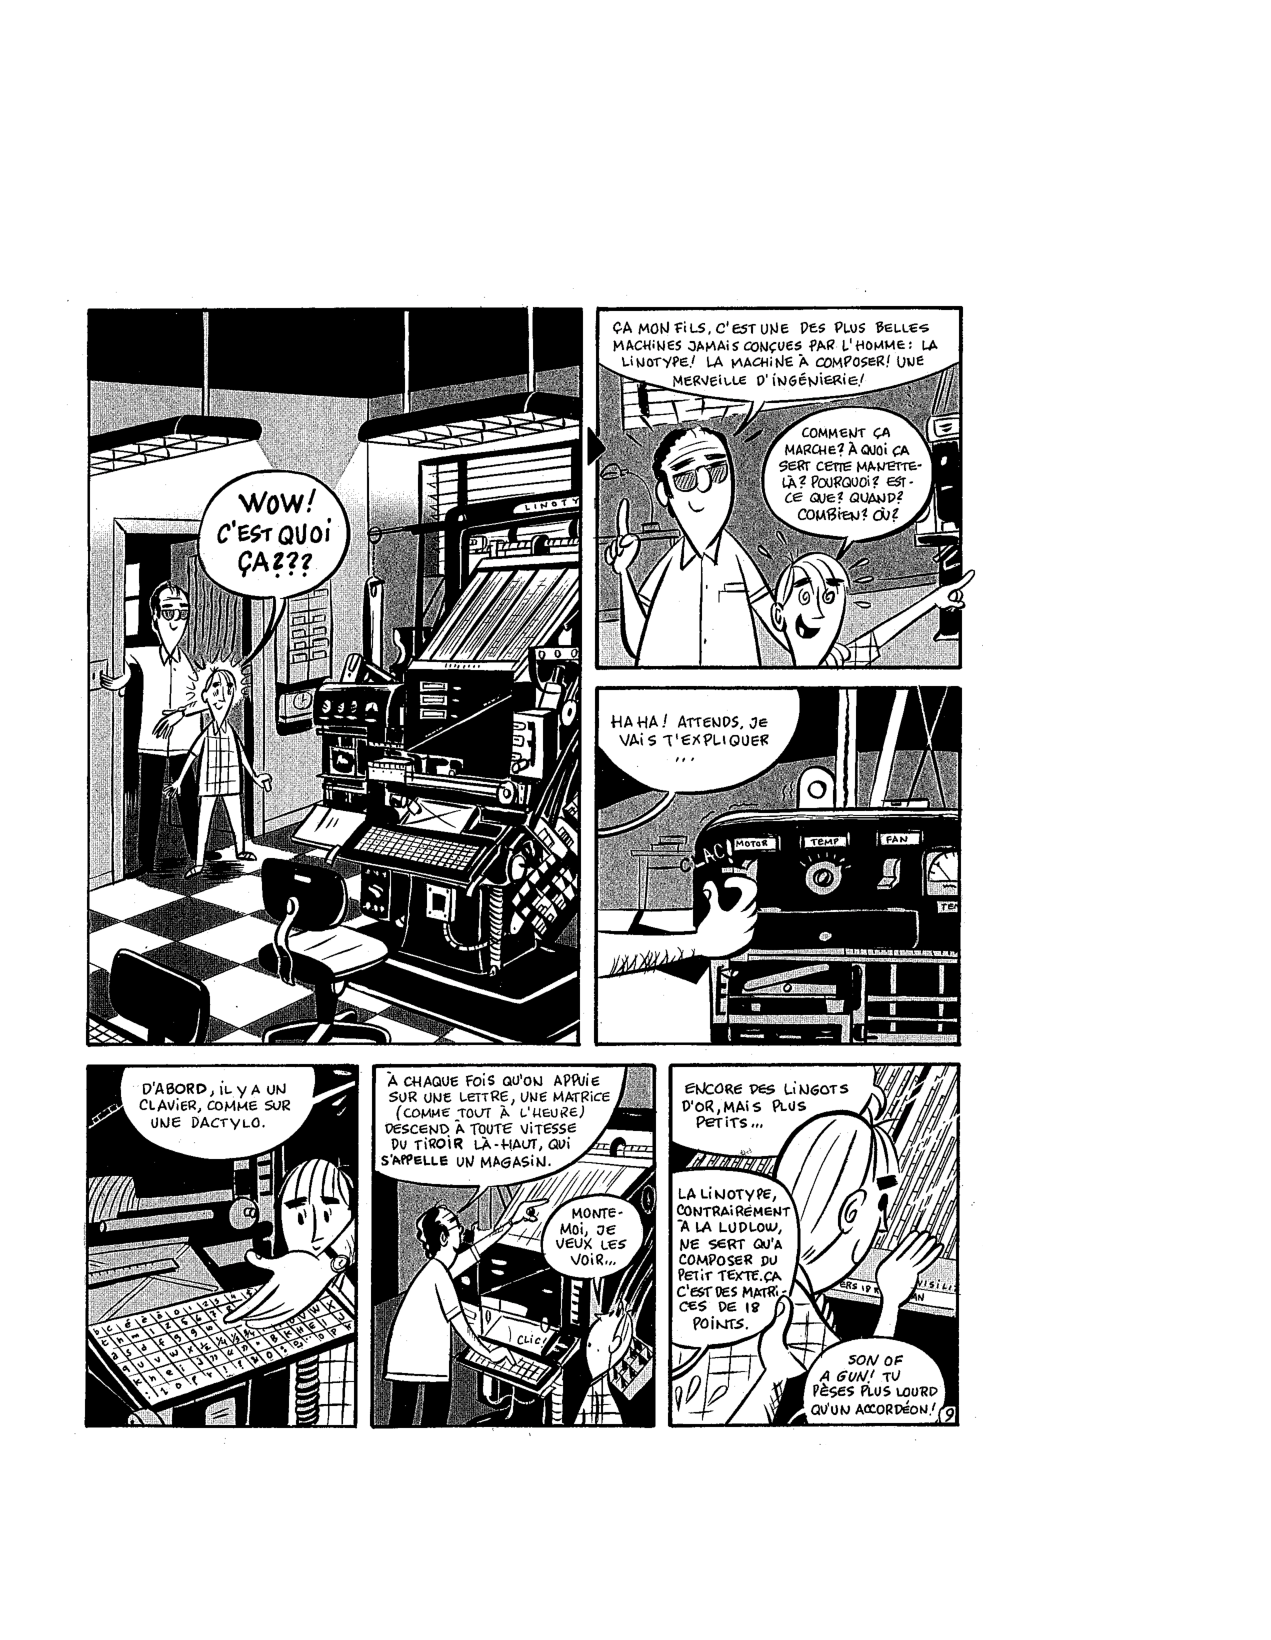
\includegraphics[angle=180]{paul-apprenti-typographe/paul-page_1}
\end{textblock*}
\begin{textblock*}{440pt}(80pt,-5pt)
  \small\sffamily%
  Extraits de «Paul à la campagne», {\textcopyright} Michel
  Rabagliati, 1999.
\end{textblock*}
\begin{textblock*}{110pt}(-40pt,-60pt)
  
\includegraphics[angle=180]{paul-apprenti-typographe/paul-titre}
\end{textblock*}
\null\clearpage

\begin{textblock*}{440pt}(0pt,0pt)
  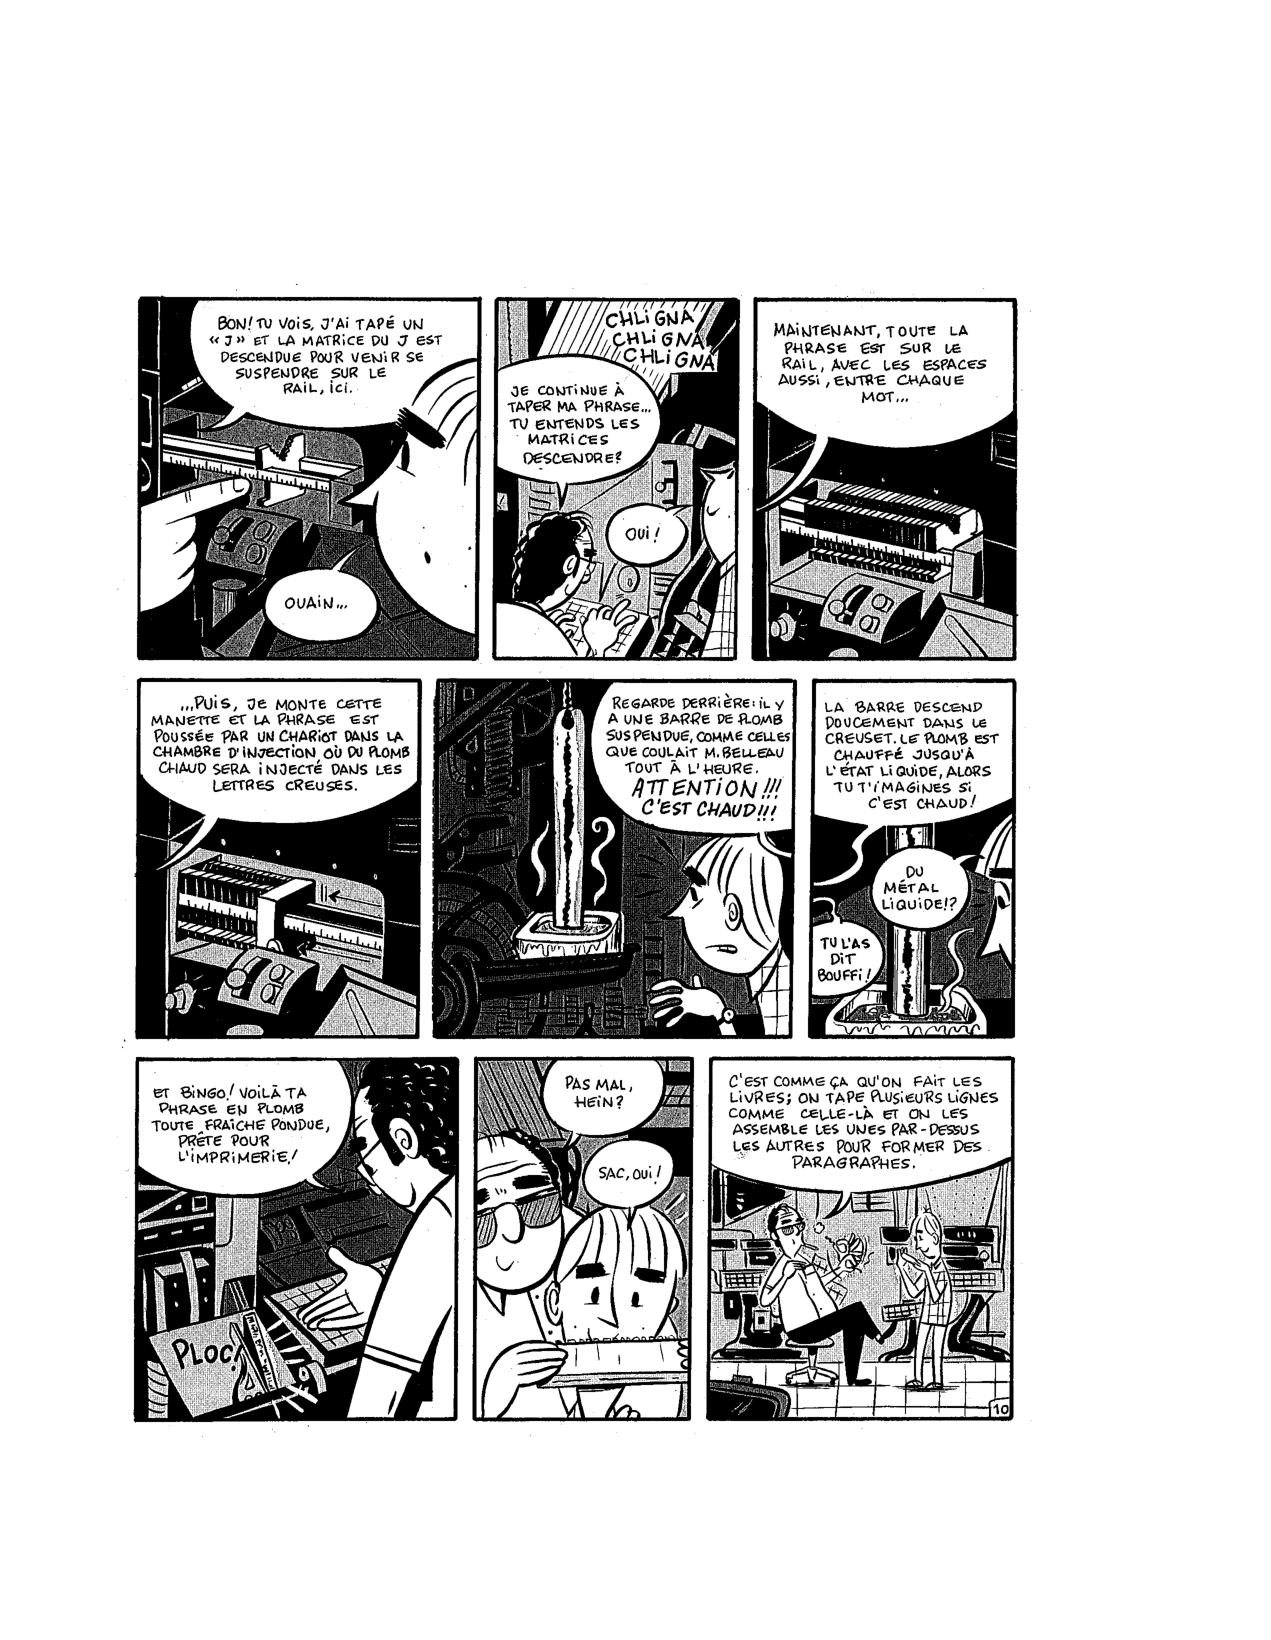
\includegraphics[angle=180]{paul-apprenti-typographe/paul-page_2}
\end{textblock*}
\null\clearpage

\begin{textblock*}{440pt}(0pt,0pt)
  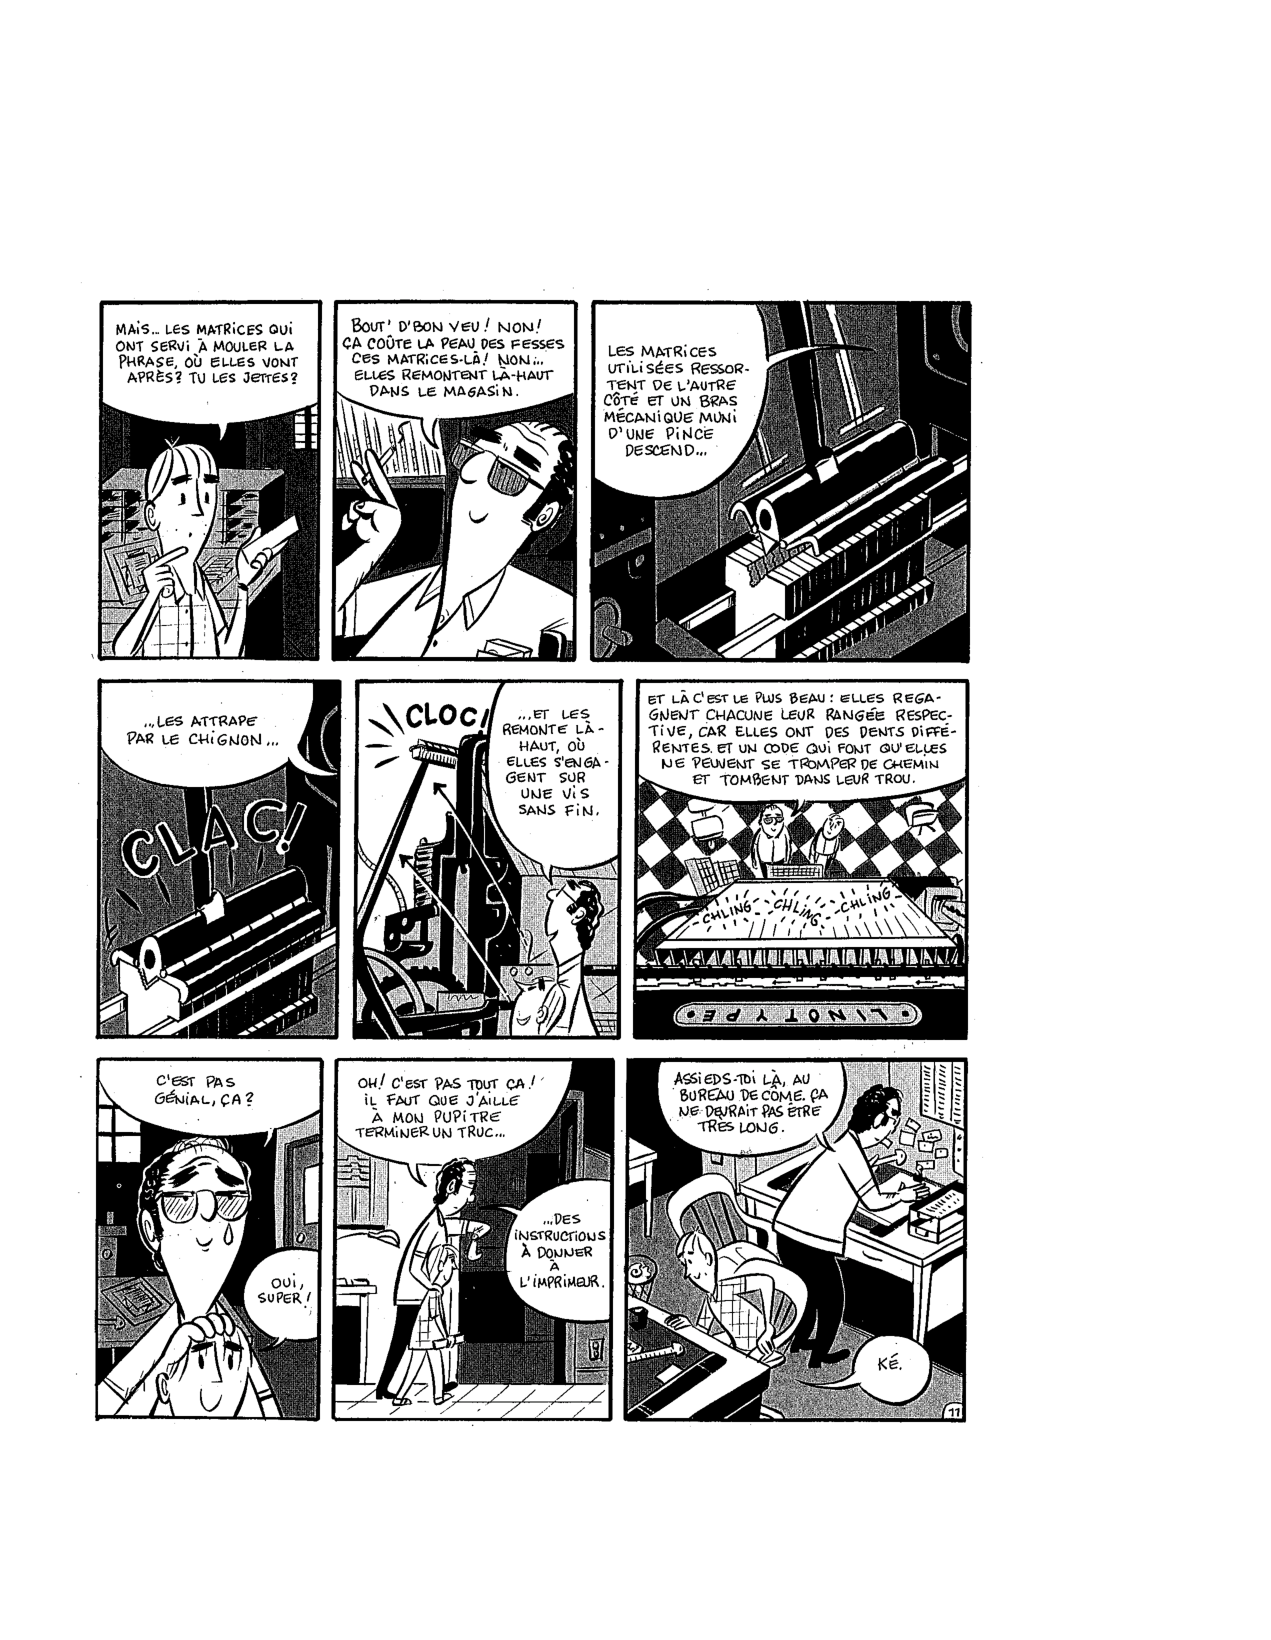
\includegraphics[angle=180]{paul-apprenti-typographe/paul-page_3}
\end{textblock*}
\null\clearpage

\begin{textblock*}{440pt}(0pt,0pt)
  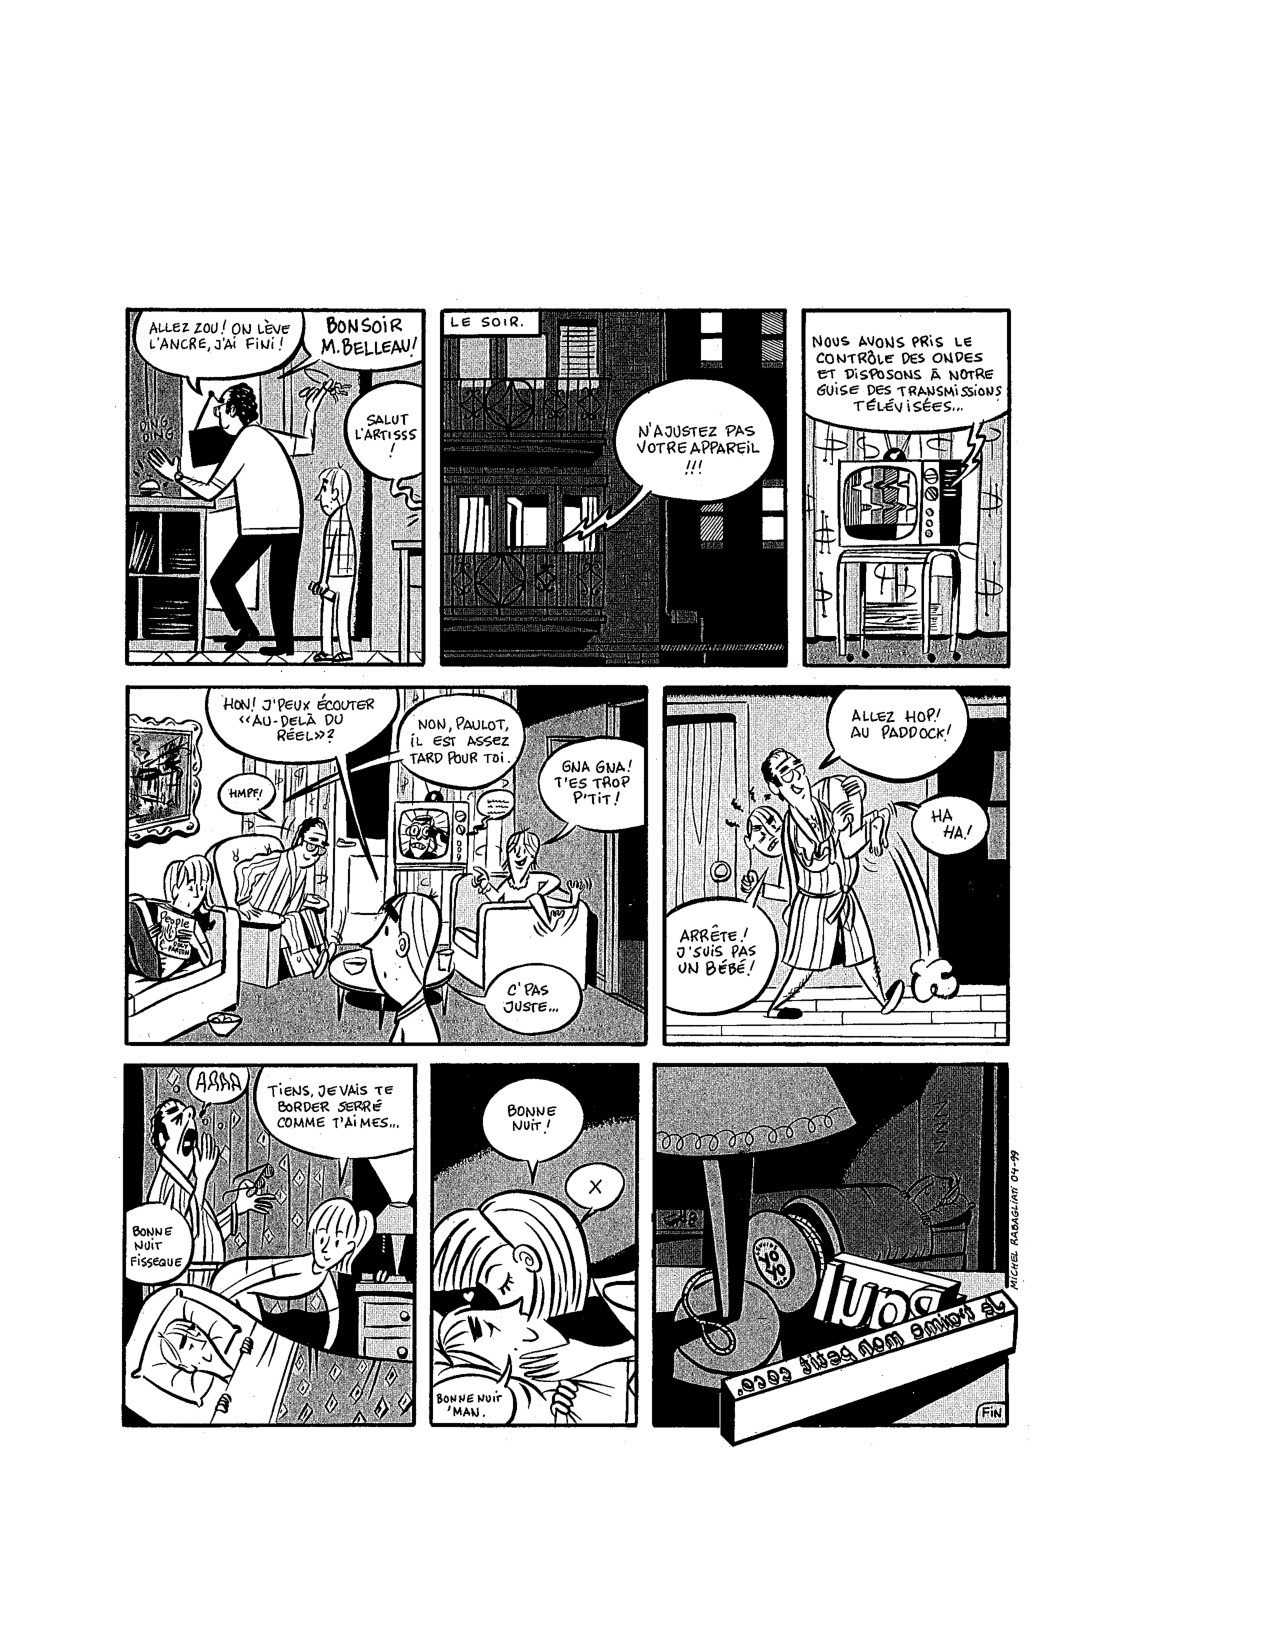
\includegraphics[angle=180]{paul-apprenti-typographe/paul-page_4}
\end{textblock*}
\null\clearpage
\endgroup

%%% Local Variables:
%%% mode: latex
%%% TeX-master: "formation-latex-ul"
%%% TeX-engine: xetex
%%% coding: utf-8
%%% End:
